\documentclass[11pt,letterpaper]{article}

% ==============================================================================
% PAQUETES Y CONFIGURACIÓN BÁSICA
% ==============================================================================
\usepackage[utf8]{inputenc}
\usepackage[T1]{fontenc}
\usepackage[spanish,es-nodecimaldot]{babel}
\usepackage{amsmath,amssymb}
\usepackage{graphicx}
\usepackage[letterpaper,top=2.2cm,bottom=2.2cm,left=2.2cm,right=2.2cm]{geometry}
\usepackage{xcolor}
\usepackage{booktabs,tabularx,array,multirow}
\usepackage{listings}
\usepackage[most]{tcolorbox}
\usepackage{fancyhdr}
\usepackage{caption}
\usepackage{subcaption}
\usepackage{float}
\usepackage{enumitem}
\usepackage{microtype}
\usepackage{url}
\usepackage{hyperref}

% ==============================================================================
% DEFINICIÓN DE COLORES
% ==============================================================================
\definecolor{primaryBlue}{HTML}{1A365D}
\definecolor{secondaryBlue}{HTML}{2B6CB0}
\definecolor{accentOrange}{HTML}{DD6B20}
\definecolor{darkGray}{HTML}{2D3748}
\definecolor{lightGray}{HTML}{F8FAFC}
\definecolor{borderGray}{HTML}{E2E8F0}
\definecolor{tagPractice}{HTML}{2B6CB0}
\definecolor{tagProject}{HTML}{4A5568}

% ==============================================================================
% CONFIGURACIÓN DE HYPERREF
% ==============================================================================
\hypersetup{
    colorlinks=true,
    linkcolor=secondaryBlue,
    citecolor=primaryBlue,
    urlcolor=secondaryBlue,
    pdfauthor={Arturo Heredia, Diego Lopez},
    pdftitle={Reporte Técnico: Comunicación Bidireccional ESP32 y Node-RED vía MQTT},
    pdfsubject={Práctica Unidad 2: IoT Bidireccional},
    pdfkeywords={IoT, ESP32, MQTT, Node-RED, Mosquitto, Bidireccional}
}

% ==============================================================================
% ENCABEZADOS Y PIES DE PÁGINA
% ==============================================================================
\pagestyle{fancy}
\fancyhf{}
\fancyhead[L]{\small\color{darkGray}\textit{ESP32 $\longleftrightarrow$ Mosquitto $\longleftrightarrow$ Node-RED (MQTT Bidireccional)}}
\fancyhead[R]{\small\color{darkGray}\textit{Práctica U2}}
\fancyfoot[L]{\small\color{darkGray}Arturo Heredia, Diego López}
\fancyfoot[R]{\thepage}
\renewcommand{\headrulewidth}{0.5pt}
\renewcommand{\footrulewidth}{0.4pt}

% ==============================================================================
% CONFIGURACIÓN DE LISTINGS (CÓDIGO FUENTE)
% ==============================================================================
\lstdefinestyle{customcpp}{
    backgroundcolor=\color{lightGray},
    basicstyle=\ttfamily\scriptsize\color{darkGray},
    keywordstyle=\bfseries\color{primaryBlue},
    commentstyle=\itshape\color{gray},
    stringstyle=\color{accentOrange},
    numbers=none,
    tabsize=2,
    showstringspaces=false,
    breaklines=true,
    frame=single,
    rulecolor=\color{borderGray},
    xleftmargin=6pt,
    framexleftmargin=6pt
}

\lstdefinestyle{custombash}{
    backgroundcolor=\color{lightGray},
    basicstyle=\ttfamily\scriptsize\color{darkGray},
    keywordstyle=\bfseries\color{secondaryBlue},
    commentstyle=\itshape\color{gray},
    stringstyle=\color{accentOrange},
    frame=single,
    rulecolor=\color{borderGray},
    breaklines=true,
    showstringspaces=false,
    xleftmargin=6pt,
    framexleftmargin=6pt
}

\lstset{style=customcpp}

% ==============================================================================
% CAJAS Y DISTINTIVOS
% ==============================================================================
\newtcolorbox{infobox}[1][]{
    colback=lightGray,
    colframe=secondaryBlue,
    arc=2mm,
    boxrule=0.8pt,
    title=#1,
    coltitle=white,
    fonttitle=\bfseries\small,
    left=3mm, right=3mm, top=2mm, bottom=2mm
}

\newcommand{\practicaBadge}{\textbf{\color{tagPractice}[Requerimiento Práctica] }}
\newcommand{\proyectoBadge}{\textbf{\color{tagProject}[Contexto de Proyecto] }}

% ==============================================================================
% CUERPO PRINCIPAL DEL DOCUMENTO
% ==============================================================================
\begin{document}

% 1. PORTADA
\begin{titlepage}
    \centering
    \vspace*{1.0cm}
    
    {\scshape\Large Universidad / Instituto Tecnológico \par}
    \vspace{0.3cm}
    {\scshape\large Asignatura: Internet de las Cosas (IoT) / Sistemas Embebidos \par}
    \vspace{0.2cm}
    {\large Unidad 2: Comunicación Bidireccional IoT \par}
    
    \vspace{2.0cm}
    
    \begin{tcolorbox}[colback=primaryBlue,colframe=primaryBlue,arc=2mm,center,width=0.95\textwidth]
        \centering\color{white}
        \vspace{0.3cm}
        {\LARGE\bfseries REPORTE TÉCNICO \par}
        \vspace{0.25cm}
        {\Large Comunicación Bidireccional entre ESP32 y Node-RED mediante Protocolo MQTT \par}
        \vspace{0.2cm}
        {\small Telemetría de Temperatura/Humedad, Control de Actuador LED y Supervisión LWT \par}
        \vspace{0.3cm}
    \end{tcolorbox}
    
    \vspace{2.5cm}
    
    \begin{minipage}[t]{0.85\textwidth}
        \centering \large
        \textbf{Autores:}\\
        \vspace{0.2cm}
        {\Large Arturo Heredia \quad \textbar \quad Diego López}
    \end{minipage}
    
    \vspace{2.5cm}
    
    \begin{infobox}[Código Fuente y Recursos]
        \centering\small
        Repositorio GitHub: \textbf{\url{https://github.com/arturoherediam/esp32-monitoreo-ambiental-iot}}
    \end{infobox}
    
    \vfill
    
    {\large Octubre de 2026 \par}
\end{titlepage}


% ÍNDICE COMPACTO
\newpage
\pagenumbering{roman}
\tableofcontents
\newpage
\pagenumbering{arabic}

% 2. OBJETIVO
\section{Objetivo}

\subsection{Objetivo de la Práctica}
Desarrollar un sistema IoT que establezca una \textbf{comunicación bidireccional} entre una placa \textbf{ESP32} y una interfaz en \textbf{Node-RED} utilizando el protocolo \textbf{MQTT}:
\begin{itemize}[noitemsep]
    \item \textbf{Sentido ascendente (ESP32 $\to$ Node-RED):} Adquisición periódica y publicación de temperatura y humedad ambiental hacia tópicos independientes.
    \item \textbf{Sentido descendente (Node-RED $\to$ ESP32):} Envío de comandos remotos desde un Dashboard web para conmutar un actuador (LED) y confirmación de su estado real.
\end{itemize}

\subsection{Relación con el Proyecto Base y Alcance}
\begin{itemize}[noitemsep]
    \item \practicaBadge Comunicación bidireccional MQTT, publicación de variables de temperatura y humedad, control de LED con confirmación de estado, broker Mosquitto y Dashboard gráfico en Node-RED.
    \item \proyectoBadge El sistema forma parte de un monitor de confort térmico que complementa la práctica integrando una pantalla local OLED (SSD1306), sensor I²C de alta precisión SHT41 (sustituto del DHT11 y relevo del BME680 inicial), y control de acceso por roles (ACL).
\end{itemize}

\subsection{Requerimientos Funcionales}
En la Tabla~\ref{tab:req_funcionales} se resume el cumplimiento de los 10 requerimientos funcionales solicitados.

\begin{table}[H]
\centering
\small
\begin{tabularx}{\textwidth}{c p{6.0cm} X c}
\toprule
\textbf{\#} & \textbf{Requerimiento de la Práctica} & \textbf{Implementación} & \textbf{Estado} \\
\midrule
1 & Conexión de ESP32 a Wi-Fi & Modo estación (\texttt{WIFI\_STA}) en hotspot local WPA2 & \textbf{Cumplido} \\
2 & Comunicación con broker MQTT & Cliente \texttt{PubSubClient} con autenticación en puerto 1883 & \textbf{Cumplido} \\
3 & Obtención de temperatura y humedad & Sensor ambiental digital con lecturas cada 2 s & \textbf{Cumplido} \\
4 & Publicación de valores vía MQTT & Tópicos dedicados \texttt{sensor/sht41/temperatura} y \texttt{humedad} & \textbf{Cumplido} \\
5 & Recepción y visualización en Node-RED & Nodos \texttt{mqtt in} conectados a Mosquitto (\texttt{localhost}) & \textbf{Cumplido} \\
6 & Interfaz gráfica (Dashboard) & Gauges analógicos y tendencias temporales en Dashboard 2.0 & \textbf{Cumplido} \\
7 & Comando para controlar el LED & Switch web que publica en \texttt{actuador/led/set} (QoS 1, retain) & \textbf{Cumplido} \\
8 & Recepción del comando en ESP32 & Callback asíncrono MQTT que decodifica órdenes \texttt{ON}/\texttt{OFF} & \textbf{Cumplido} \\
9 & Conmutación física del LED & \texttt{digitalWrite(GPIO 2)} con encendido simultáneo de onboard & \textbf{Cumplido} \\
10 & Comunicación bidireccional & Lazo cerrado con confirmación en \texttt{actuador/led/estado} y LWT & \textbf{Cumplido} \\
\bottomrule
\end{tabularx}
\caption{Matriz de cumplimiento de requerimientos funcionales.}
\label{tab:req_funcionales}
\end{table}


% 3. MATERIALES
\section{Materiales}

\subsection{Lista de Materiales de la Práctica}
En la Tabla~\ref{tab:materiales} se desglosan los materiales solicitados para la práctica y los componentes equivalentes o adicionales implementados en el proyecto.

\begin{table}[H]
\centering
\small
\begin{tabularx}{\textwidth}{c p{3.2cm} p{4.0cm} X c}
\toprule
\textbf{\#} & \textbf{Requerido en Guía} & \textbf{Componente Utilizado} & \textbf{Función y Justificación} & \textbf{Cant.} \\
\midrule
1 & 1 ESP32 & ESP32 DevKit V1 (30 pines) & Microcontrolador con Wi-Fi, cliente MQTT y GPIO. & 1 \\
2 & 1 Sensor DHT11 & Sensor digital GY-SHT41 \newline \textit{(Sensirion SHT41, I²C)} & Mide temperatura ($\pm 0.2\,^\circ\text{C}$) y humedad ($\pm 1.8\%$). Supera al DHT11 y usa bus estándar I²C. & 1 \\
3 & 1 LED & LED difuso de 5 mm rojo & Actuador conmutable conectado a GPIO 2. & 1 \\
4 & Resistencias & Resistor $220\,\Omega$, $1/4\,\text{W}$ & Limitador de corriente de polarización del LED. & 1 \\
5 & Protoboard & Protoboard de 830 puntos & Placa de pruebas para el montaje sin soldadura. & 1 \\
6 & Cables & Jumpers macho-macho & Conexiones de bus I²C, GPIO, 3.3V y GND. & $\sim 12$ \\
7 & Computadora e Internet & Laptop con Linux (hotspot) & Alojamiento de Mosquitto broker y Node-RED. & 1 \\
\midrule
\multicolumn{5}{l}{\proyectoBadge \textbf{Componentes adicionales incorporados en el proyecto:}} \\
8 & Pantalla local & OLED 128$\times$32 SSD1306 (I²C) & Muestra temp/humedad y estado del LED in situ. & 1 \\
\bottomrule
\end{tabularx}
\caption{Lista de materiales requeridos y componentes utilizados.}
\label{tab:materiales}
\end{table}

\subsection{Distinción Técnica: DHT11 frente a SHT41 y Diagnóstico BME680}
\begin{itemize}
    \item \practicaBadge \textbf{Sensor de Temperatura y Humedad:} La guía solicita un DHT11 (protocolo propietario 1-wire, resolución de 8 bits, precisión $\pm 2^\circ\text{C}$ / $\pm 5\%$). En este trabajo se optó por el sensor digital \textbf{SHT41} de Sensirion por su protocolo estándar I²C (dirección \texttt{0x44}), resolución de 16 bits ($\pm 0.2^\circ\text{C}$ / $\pm 1.8\%$) y operación no bloqueante en el microcontrolador.
    \item \proyectoBadge \textbf{Antecedente del BME680:} Inicialmente se probó un sensor BME680 (temperatura, humedad, presión y gas). Durante las pruebas diagnósticas se constató que su registro interno de temperatura arrojaba invariablemente \texttt{adc\_T = 0} por falla de fabricación en el silicio, por lo que fue sustituido por el SHT41, focalizando el proyecto en confort térmico.
\end{itemize}


% 4. DIAGRAMA DE CONEXIÓN
\section{Diagrama de Conexión}

\subsection{Esquemático del Circuito}
El conexionado físico del sistema optimiza el uso de terminales utilizando un bus I²C compartido y una salida digital para el actuador, como se muestra en la Figura~\ref{fig:diagrama_conexiones}.

\begin{figure}[H]
    \centering
    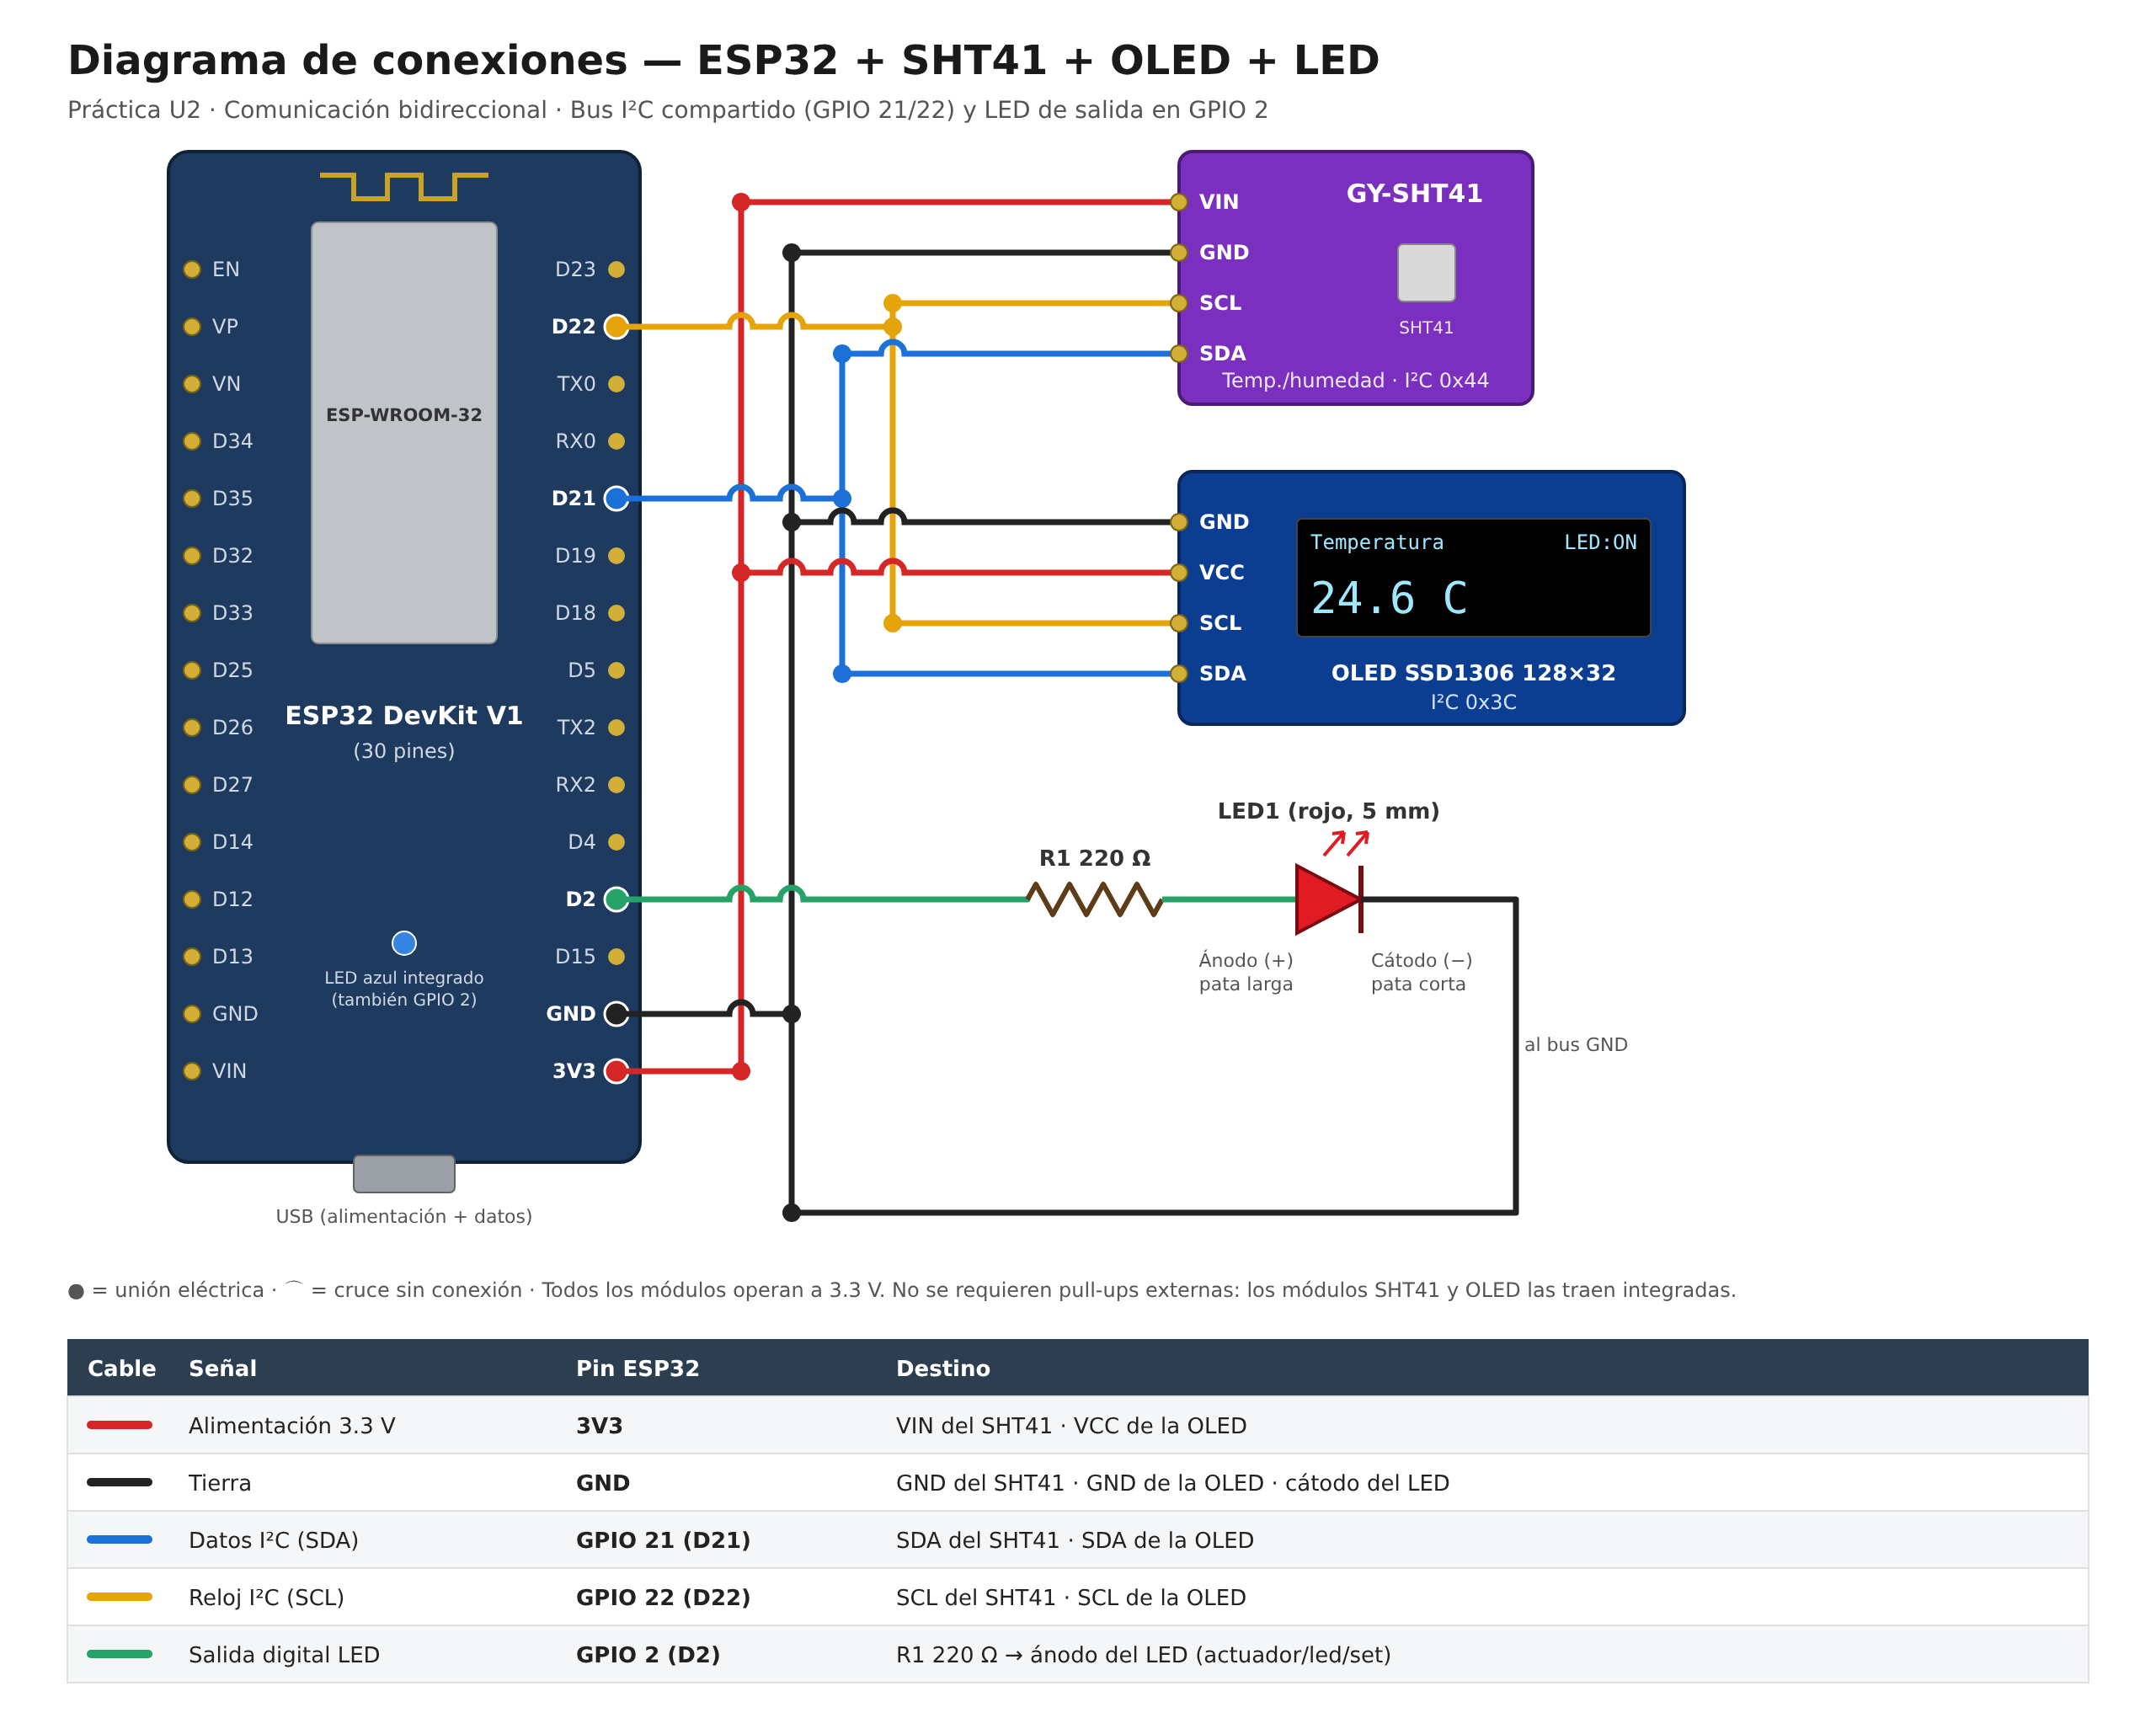
\includegraphics[width=0.92\textwidth]{imagenes/diagrama_conexiones.png}
    \caption{Diagrama de conexión: ESP32 DevKit V1, sensor ambiental SHT41, pantalla OLED y LED en GPIO 2.}
    \label{fig:diagrama_conexiones}
\end{figure}

\subsection{Asignación de Terminales y Conexiones}
\begin{table}[H]
\centering
\small
\begin{tabularx}{\textwidth}{l c l X}
\toprule
\textbf{Señal} & \textbf{Pin ESP32} & \textbf{Destino Físico} & \textbf{Categoría / Propósito} \\
\midrule
\texttt{3V3} & 3V3 & \texttt{VIN} de SHT41 y \texttt{VCC} de OLED & Alimentación lógica regulada (3.3V). \\
\texttt{GND} & GND & \texttt{GND} de SHT41, OLED y cátodo del LED & Referencia común de tierra. \\
\texttt{GPIO 21} & D21 (SDA) & \texttt{SDA} de SHT41 y \texttt{SDA} de OLED & Línea de datos I²C compartida. \\
\texttt{GPIO 22} & D22 (SCL) & \texttt{SCL} de SHT41 y \texttt{SCL} de OLED & Reloj I²C (100 kHz). \\
\texttt{GPIO 2} & D2 & Resistor $220\,\Omega$ $\to$ ánodo LED & \practicaBadge Salida del actuador conmutable. \\
\bottomrule
\end{tabularx}
\caption{Mapeo de pines del circuito.}
\label{tab:pinout}
\end{table}

\subsection{Cálculo Eléctrico del Circuito del LED}
Para un nivel lógico alto en el ESP32 ($V_{OH} \approx 3.3\,\text{V}$) y una caída de tensión típica del LED rojo ($V_F \approx 2.0\,\text{V}$), la corriente de polarización es:
\begin{equation}
    I_{LED} = \frac{V_{OH} - V_F}{R} = \frac{3.3\,\text{V} - 2.0\,\text{V}}{220\,\Omega} = 5.91\,\text{mA}
\end{equation}
La potencia disipada en el resistor es $P = I_{LED}^2 \cdot R \approx 7.68\,\text{mW}$ (muy inferior a la capacidad nominal de $250\,\text{mW}$). La corriente de $5.91\,\text{mA}$ está dentro del límite seguro del pin del ESP32 ($\le 12\,\text{mA}$).

\paragraph{Nota de diseño (Strapping Pin y LED integrado):} El pin \texttt{GPIO 2} es un pin de configuración de arranque (\textit{boot strapping}); la resistencia a GND mantiene el pin en nivel bajo durante el encendido sin interferir con el arranque ni la programación. Además, \texttt{GPIO 2} conmuta en paralelo el LED azul integrado en la placa DevKit.


% 5. ARQUITECTURA DEL SISTEMA
\section{Arquitectura del Sistema}

\subsection{Estructura General y Comunicación IoT}
El sistema se organiza en tres capas jerárquicas interconectadas mediante el protocolo MQTT, como se ilustra en la Figura~\ref{fig:diagrama_arquitectura}:
\begin{enumerate}[noitemsep]
    \item \textbf{Capa de Percepción (ESP32):} Adquisición de magnitudes físicas, control de salida digital y cliente MQTT (\texttt{PubSubClient}).
    \item \textbf{Capa de Transporte (Red local + Mosquitto):} Enlace inalámbrico Wi-Fi y servidor de mensajería MQTT (puerto 1883).
    \item \textbf{Capa de Aplicación (Node-RED):} Flujo de eventos y panel gráfico interactivo en Dashboard 2.0.
\end{enumerate}

\begin{figure}[H]
    \centering
    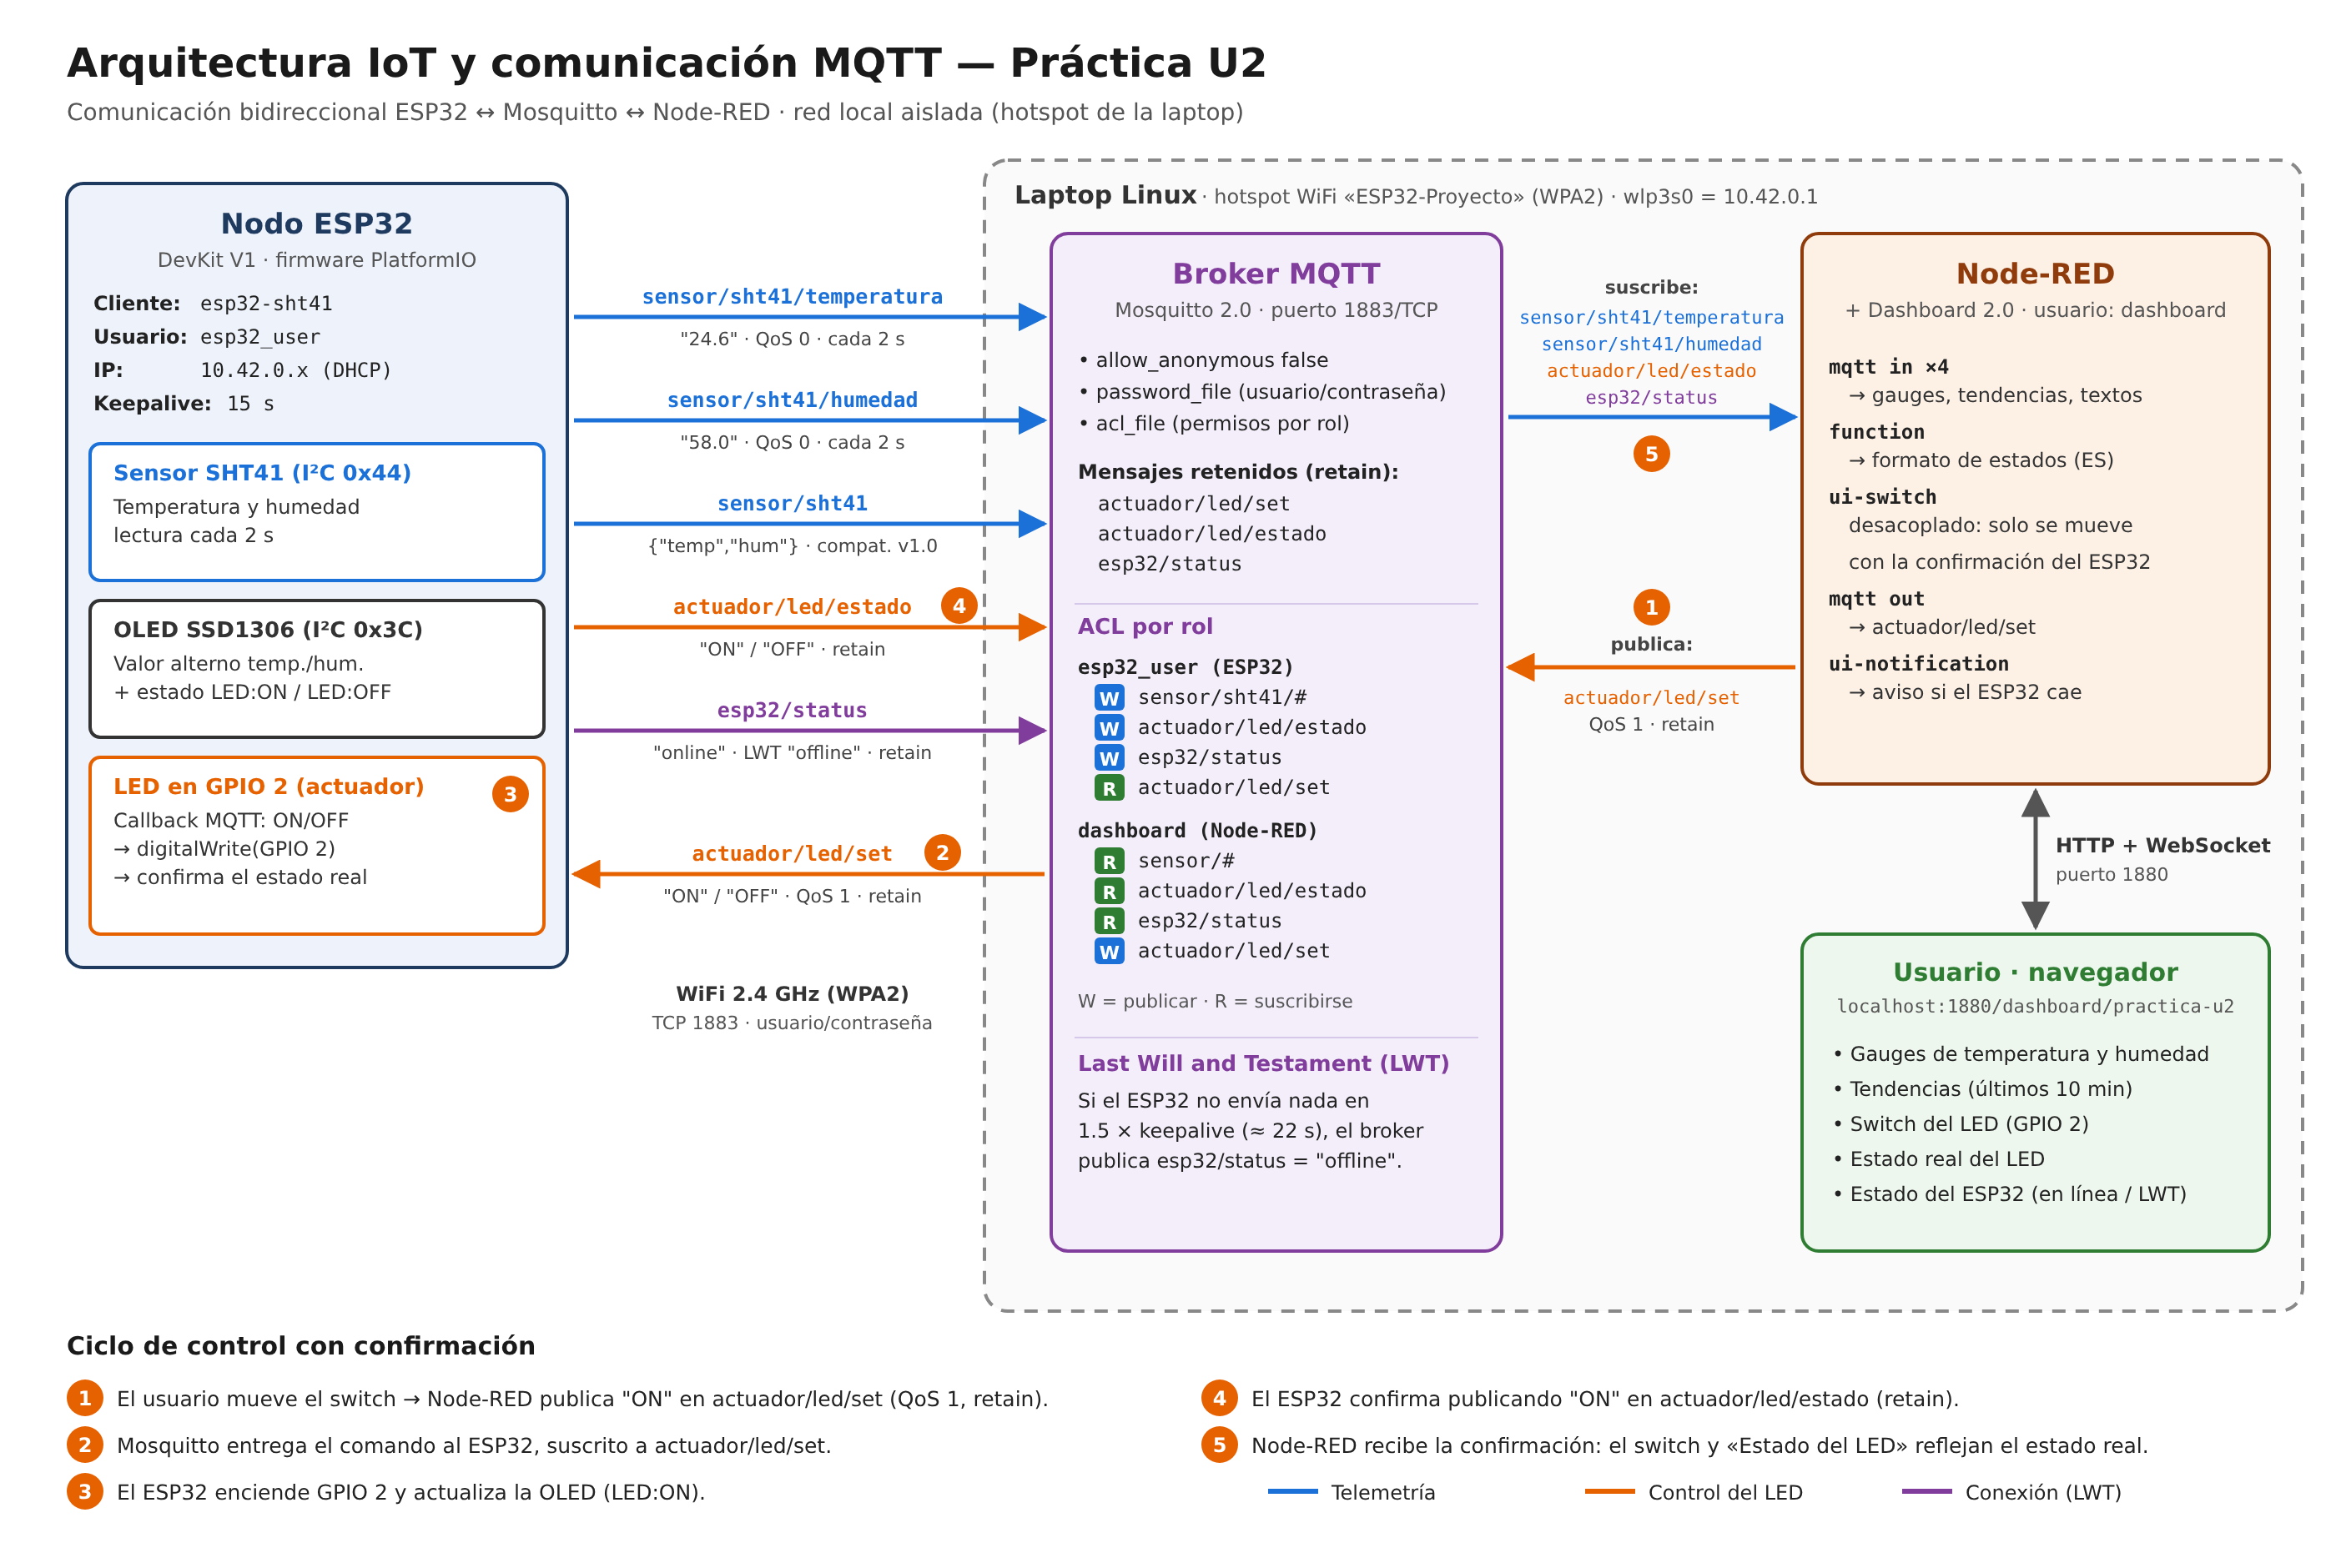
\includegraphics[width=0.96\textwidth]{imagenes/diagrama_arquitectura.png}
    \caption{Arquitectura general del sistema, red local y comunicación bidireccional MQTT.}
    \label{fig:diagrama_arquitectura}
\end{figure}

\subsection{Configuración de Red Local (Hotspot)}
\begin{itemize}[noitemsep]
    \item \practicaBadge \textbf{Enlace Wi-Fi:} La ESP32 se conecta como estación (\texttt{WIFI\_STA}) al punto de acceso local bajo cifrado WPA2.
    \item \proyectoBadge \textbf{Red Aislada de Laboratorio:} La laptop genera el punto de acceso mediante NetworkManager (\texttt{nmcli}), asignando una subred privada fija \texttt{10.42.0.0/24} con IP del broker en \texttt{10.42.0.1}. Esto aísla el tráfico de redes institucionales y asegura que el puerto 1883 no sufra bloqueos de cortafuegos externos.
\end{itemize}


% 6. DESCRIPCIÓN DEL FUNCIONAMIENTO
\section{Descripción del Funcionamiento}

\subsection{Flujo Operativo de la Práctica}
El sistema opera en ciclo continuo sin funciones bloqueantes (\texttt{millis()}):
\begin{enumerate}
    \item \textbf{Inicialización:} Al encenderse, el ESP32 inicializa el bus I²C, el sensor y la salida del LED (\texttt{LOW} por defecto). Establece conexión con el punto de acceso Wi-Fi y con el broker Mosquitto.
    \item \textbf{Telemetría periódica (2 segundos):} Cada $2000\,\text{ms}$, el ESP32 lee la temperatura ($^\circ\text{C}$) y humedad ($\%$) y las publica en los tópicos independientes \texttt{sensor/sht41/temperatura} y \texttt{sensor/sht41/humedad}.
    \item \textbf{Visualización en Dashboard:} Node-RED recibe las lecturas y las representa en tiempo real en los medidores radiales (\textit{gauges}) e historiales gráficos.
    \item \textbf{Control de Actuador (Lazo Cerrado):} El usuario activa el interruptor en el Dashboard; Node-RED envía \texttt{"ON"} a \texttt{actuador/led/set}. El ESP32 recibe la orden, enciende el LED físico en \texttt{GPIO 2} y publica la confirmación \texttt{"ON"} en \texttt{actuador/led/estado}.
\end{enumerate}

\subsection{Ciclo de Control con Confirmación de Estado}
Para evitar que la interfaz muestre estados erróneos si el dispositivo pierde conexión o energía, el switch de Node-RED está configurado en modo \textbf{desacoplado}: la perilla gráfica solo cambia de posición cuando el ESP32 devuelve la confirmación física, como se describe en la Figura~\ref{fig:ciclo_control}.

\begin{figure}[H]
    \centering
    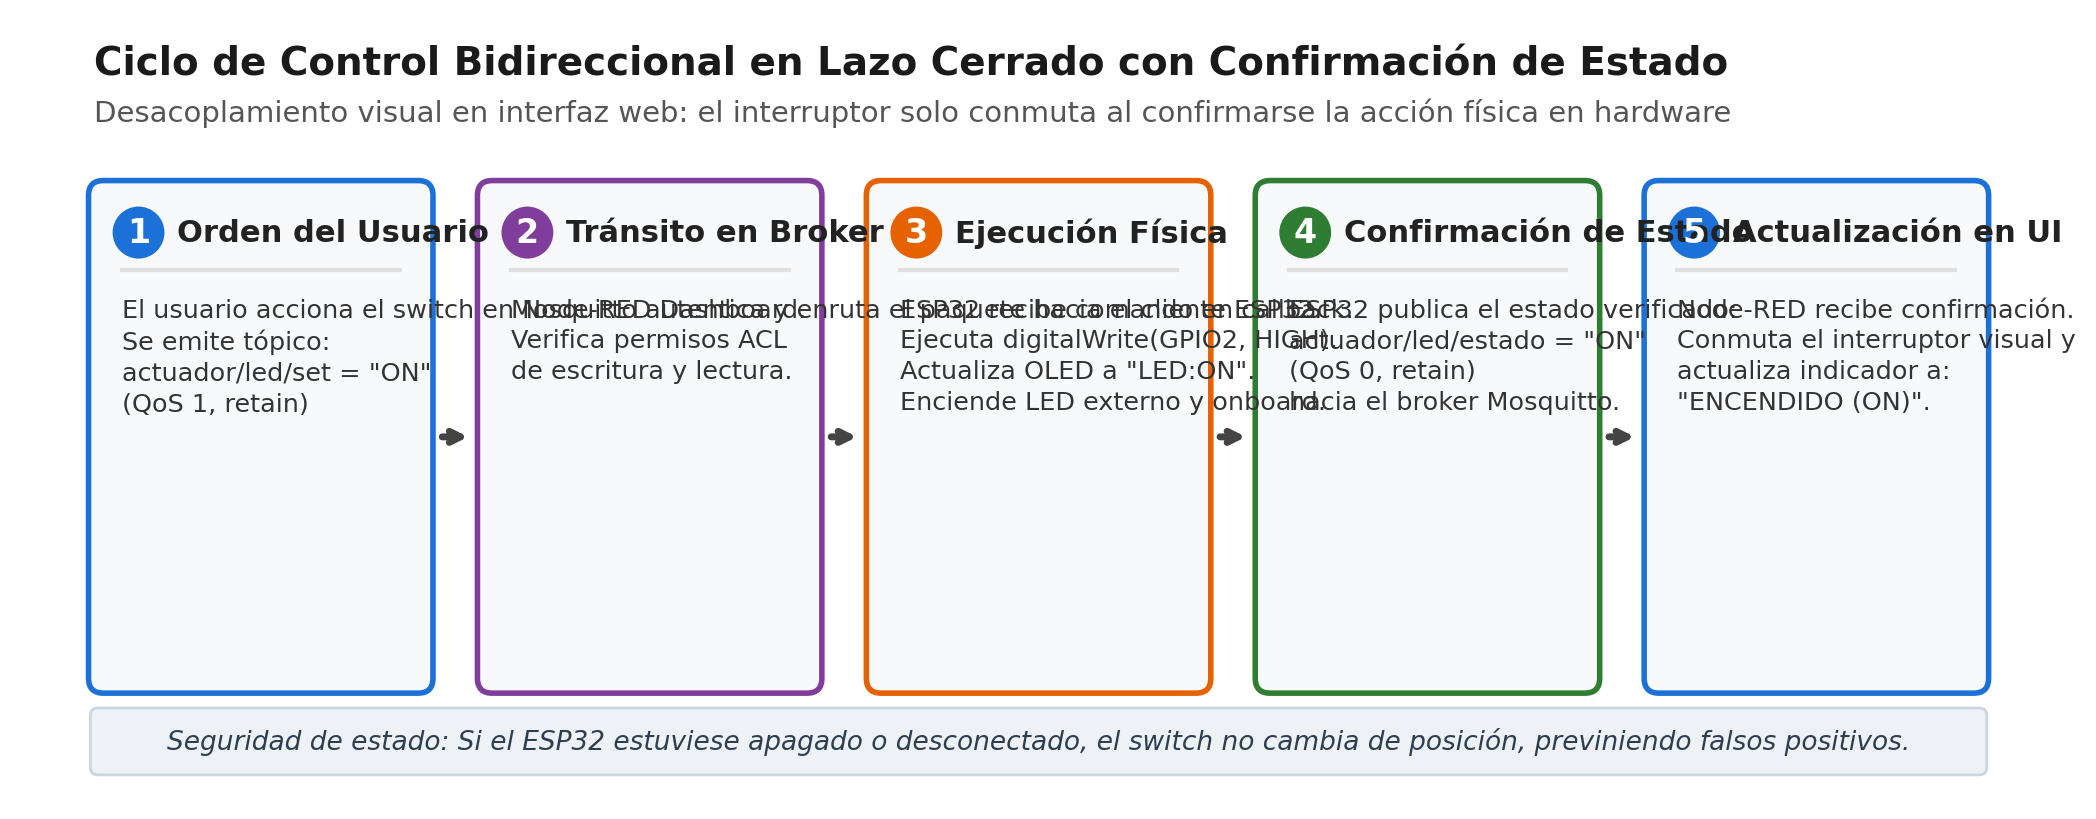
\includegraphics[width=0.96\textwidth]{imagenes/ciclo_control_closed_loop.png}
    \caption{Secuencia de control bidireccional en lazo cerrado con confirmación y desacoplamiento.}
    \label{fig:ciclo_control}
\end{figure}

\subsection{Supervisión de Disponibilidad mediante LWT (\textit{Last Will and Testament})}
\begin{itemize}[noitemsep]
    \item \practicaBadge \textbf{Detección de desconexión:} Al conectarse, el microcontrolador registra en Mosquitto el mensaje \texttt{esp32/status = "offline"} como última voluntad. Una vez enlazado, publica \texttt{"online"}.
    \item Si el ESP32 sufre un corte de energía o pierde señal por más de $1.5 \times \text{keepalive} \approx 22\,\text{s}$, el broker publica automáticamente \texttt{"offline"}. Node-RED detecta el cambio, muestra el estado \textbf{🔴 Desconectado} y despliega una notificación de alerta.
    \item \proyectoBadge \textbf{Visualización local y retención:} La pantalla OLED refleja de inmediato el estado del LED (\texttt{LED:ON} / \texttt{LED:OFF}). Al reconectar tras un reinicio, el ESP32 lee el comando retenido en el broker y restaura el estado del actuador sin intervención del usuario.
\end{itemize}


% 7. CONFIGURACIÓN MQTT
\section{Configuración MQTT y Seguridad}

\subsection{Parámetros del Broker MQTT}
En la Tabla~\ref{tab:config_broker} se detallan los parámetros de conexión del broker de mensajería implementado.

\begin{table}[H]
\centering
\small
\begin{tabularx}{\textwidth}{l p{4.5cm} X}
\toprule
\textbf{Parámetro} & \textbf{Valor} & \textbf{Descripción / Uso} \\
\midrule
\textbf{Software Broker} & Eclipse Mosquitto v2.0.x & Servidor de mensajería MQTT en GNU/Linux. \\
\textbf{Dirección IP} & \texttt{10.42.0.1} (WLAN) / \texttt{localhost} & IP del servidor para el ESP32 y para Node-RED. \\
\textbf{Puerto} & \texttt{1883/TCP} & Puerto estándar para tráfico MQTT en texto plano. \\
\textbf{Acceso Anónimo} & Desactivado (\texttt{allow\_anonymous false}) & Requiere autenticación por usuario y contraseña. \\
\textbf{Usuarios del Sistema} & \texttt{esp32\_user} y \texttt{dashboard} & Roles diferenciados para nodo de campo y servidor web. \\
\bottomrule
\end{tabularx}
\caption{Parámetros de configuración del broker MQTT.}
\label{tab:config_broker}
\end{table}

\subsection{Autenticación y Credenciales}
En el archivo \texttt{/etc/mosquitto/conf.d/local.conf} se establecieron las directivas de escucha y autenticación:
\begin{lstlisting}[style=custombash]
listener 1883 0.0.0.0
allow_anonymous false
password_file /etc/mosquitto/passwd
acl_file /etc/mosquitto/acl
\end{lstlisting}
Los usuarios se dieron de alta mediante \texttt{sudo mosquitto\_passwd /etc/mosquitto/passwd <usuario>}.

\subsection{Control de Acceso por Roles (ACL) y Firewall}
\begin{itemize}
    \item \proyectoBadge \textbf{Listas de Control de Acceso (ACL):} En \texttt{/etc/mosquitto/acl} se delimitaron los privilegios mínimos para aislar funciones:
    \begin{itemize}[noitemsep]
        \item \texttt{esp32\_user}: Permiso de escritura en \texttt{sensor/sht41/\#}, \texttt{actuador/led/estado} y \texttt{esp32/status}; permiso de lectura únicamente en \texttt{actuador/led/set}.
        \item \texttt{dashboard}: Permiso de lectura en \texttt{sensor/\#}, \texttt{actuador/led/estado} y \texttt{esp32/status}; permiso de escritura únicamente en \texttt{actuador/led/set}.
    \end{itemize}
    \item \proyectoBadge \textbf{Regla de Firewall UFW:} Se limitó el acceso al puerto 1883 exclusivamente a la subred del proyecto:
    \begin{lstlisting}[style=custombash]
sudo ufw allow from 10.42.0.0/24 to any port 1883 proto tcp
    \end{lstlisting}
\end{itemize}


% 8. TOPICS UTILIZADOS
\section{Topics Utilizados y Estructura de Mensajes}

\subsection{Matriz de Tópicos MQTT}
En la Tabla~\ref{tab:topicos_mqtt} se resumen los tópicos implementados, su dirección, formato de payload, nivel de QoS y bandera de retención.

\begin{table}[H]
\centering
\small
\begin{tabularx}{\textwidth}{p{4.2cm} c c c p{2.2cm} X}
\toprule
\textbf{Tópico MQTT} & \textbf{Flujo} & \textbf{QoS} & \textbf{Ret.} & \textbf{Payload} & \textbf{Propósito / Función} \\
\midrule
\texttt{sensor/sht41/temperatura} & ESP32 $\to$ NR & 0 & No & \texttt{"24.6"} & Lectura de temperatura en $^\circ\text{C}$ (texto ASCII). \\
\texttt{sensor/sht41/humedad} & ESP32 $\to$ NR & 0 & No & \texttt{"58.0"} & Lectura de humedad en $\%$ (texto ASCII). \\
\texttt{actuador/led/set} & NR $\to$ ESP32 & 1 & Sí & \texttt{ON} / \texttt{OFF} & Comando de conmutación emitido por el switch. \\
\texttt{actuador/led/estado} & ESP32 $\to$ NR & 0 & Sí & \texttt{ON} / \texttt{OFF} & Confirmación del estado real físico del LED. \\
\texttt{esp32/status} & ESP32/Brk $\to$ NR & 0 & Sí & \texttt{online}/\texttt{offline} & Supervisión de conexión y alerta LWT. \\
\midrule
\multicolumn{6}{l}{\proyectoBadge \textbf{Tópico de compatibilidad del proyecto base:}} \\
\texttt{sensor/sht41} & ESP32 $\to$ NR & 0 & No & JSON & \texttt{\{"temp":24.6,"hum":58.0\}} (retrocompatibilidad). \\
\bottomrule
\end{tabularx}
\caption{Especificación técnica de tópicos MQTT del sistema.}
\label{tab:topicos_mqtt}
\end{table}

\subsection{Estructura de Payloads y Calidad de Servicio (QoS)}
\begin{itemize}[noitemsep]
    \item \practicaBadge \textbf{Tópicos independientes en texto plano:} Los valores de temperatura (\texttt{"24.6"}) y humedad (\texttt{"58.0"}) se envían como cadenas atómicas simples para su consumo directo en los medidores radiales (\textit{gauges}) sin sobrecarga de decodificación.
    \item \practicaBadge \textbf{Comandos del actuador:} El tópico \texttt{actuador/led/set} emplea \textbf{QoS 1} para garantizar la entrega del comando y bandera \textbf{Retain = true} para que el microcontrolador recupere el último estado configurado si se reinicia.
    \item \practicaBadge \textbf{Confirmación de estado:} El tópico \texttt{actuador/led/estado} devuelve la confirmación con bandera retenida para que nuevos clientes web sincronicen de inmediato el estado del interruptor.
\end{itemize}


% 9. EXPLICACIÓN GENERAL DEL CÓDIGO
\section{Explicación General del Código}

\subsection{Firmware del Microcontrolador ESP32}
El firmware (\texttt{firmware/esp32-monitoreo-ambiental/src/main.cpp}) opera mediante temporizadores basados en \texttt{millis()}, evitando bloqueos por \texttt{delay()}.

\subsubsection{1. Conexión con LWT y Suscripción a Comandos}
\begin{lstlisting}[style=customcpp]
bool conectarMQTT() {
  // LWT: registra testamento "offline" en esp32/status
  bool ok = mqttClient.connect(MQTT_CLIENT_ID, MQTT_USER, MQTT_PASSWORD,
                               TOPIC_STATUS, 0, true, "offline");
  if (!ok) return false;

  mqttClient.publish(TOPIC_STATUS, "online", true);
  mqttClient.publish(TOPIC_LED_ESTADO, ledEncendido ? "ON" : "OFF", true);
  mqttClient.subscribe(TOPIC_LED_SET, 1); // Suscripcion a comandos con QoS 1
  return true;
}
\end{lstlisting}

\subsubsection{2. Callback de Recepción y Control con Confirmación}
\begin{lstlisting}[style=customcpp]
void callbackMQTT(char* topic, byte* payload, unsigned int length) {
  char msg[16];
  unsigned int n = min(length, (unsigned int)(sizeof(msg) - 1));
  for (unsigned int i = 0; i < n; i++) msg[i] = toupper((char)payload[i]);
  msg[n] = '\0';

  if (strcmp(topic, TOPIC_LED_SET) == 0) {
    if (strcmp(msg, "ON") == 0) aplicarLed(true);
    else if (strcmp(msg, "OFF") == 0) aplicarLed(false);
  }
}

void aplicarLed(bool encender) {
  ledEncendido = encender;
  digitalWrite(LED_PIN, encender ? HIGH : LOW); // Conmutacion fisica en GPIO 2

  if (mqttClient.connected()) {
    // Confirmacion de lazo cerrado (retained) hacia Node-RED
    mqttClient.publish(TOPIC_LED_ESTADO, encender ? "ON" : "OFF", true);
  }
  actualizarOled(); // Refresco in situ en la pantalla OLED
}
\end{lstlisting}

\subsubsection{3. Muestreo Periódico y Publicación de Telemetría}
\begin{lstlisting}[style=customcpp]
void leerYPublicar() {
  sensors_event_t hum_ev, temp_ev;
  if (!sht4.getEvent(&hum_ev, &temp_ev)) return;
  temperaturaActual = temp_ev.temperature;
  humedadActual = hum_ev.relative_humidity;

  if (!mqttClient.connected()) return;

  char val[12];
  snprintf(val, sizeof(val), "%.1f", temperaturaActual);
  mqttClient.publish(TOPIC_TEMPERATURA, val); // sensor/sht41/temperatura
  snprintf(val, sizeof(val), "%.1f", humedadActual);
  mqttClient.publish(TOPIC_HUMEDAD, val);     // sensor/sht41/humedad
}
\end{lstlisting}

\subsection{Flujo en Node-RED (\texttt{node-red/dashboard.json})}
El flujo de Node-RED se estructura en tres bloques funcionales:
\begin{enumerate}[noitemsep]
    \item \textbf{Telemetría ambiental:} Nodos \texttt{mqtt in} conectados a los tópicos individuales de temperatura y humedad, vinculados a dos medidores \texttt{ui-gauge} (rango $0$--$50^\circ\text{C}$ y $0$--$100\%$) y dos gráficas \texttt{ui-chart} de tendencia histórica (últimos 10 minutos).
    \item \textbf{Control del actuador LED (desacoplado):} El nodo \texttt{ui-switch} publica en \texttt{actuador/led/set} mediante un nodo \texttt{mqtt out} (QoS 1, retain). Un nodo \texttt{mqtt in} escucha \texttt{actuador/led/estado} y alimenta la entrada del switch para actualizar su posición real, además de un nodo \texttt{ui-text} que muestra \texttt{"ENCENDIDO"} o \texttt{"APAGADO"}.
    \item \textbf{Supervisión LWT:} Nodo \texttt{mqtt in} para \texttt{esp32/status} que actualiza el indicador de presencia (\texttt{"🟢 En línea"} / \texttt{"🔴 Desconectado"}) y genera una notificación emergente mediante \texttt{ui-notification} si el dispositivo cae.
\end{enumerate}


% 10. EVIDENCIAS
\section{Evidencias de Funcionamiento}

\subsection{Registro del Montaje Físico y Dashboard}
En la Figura~\ref{fig:evidencias_visuales} se presentan el esquema del prototipo físico en protoboard y la interfaz gráfica implementada en Node-RED Dashboard 2.0.

\begin{figure}[H]
    \centering
    \begin{subfigure}[b]{0.48\textwidth}
        \centering
        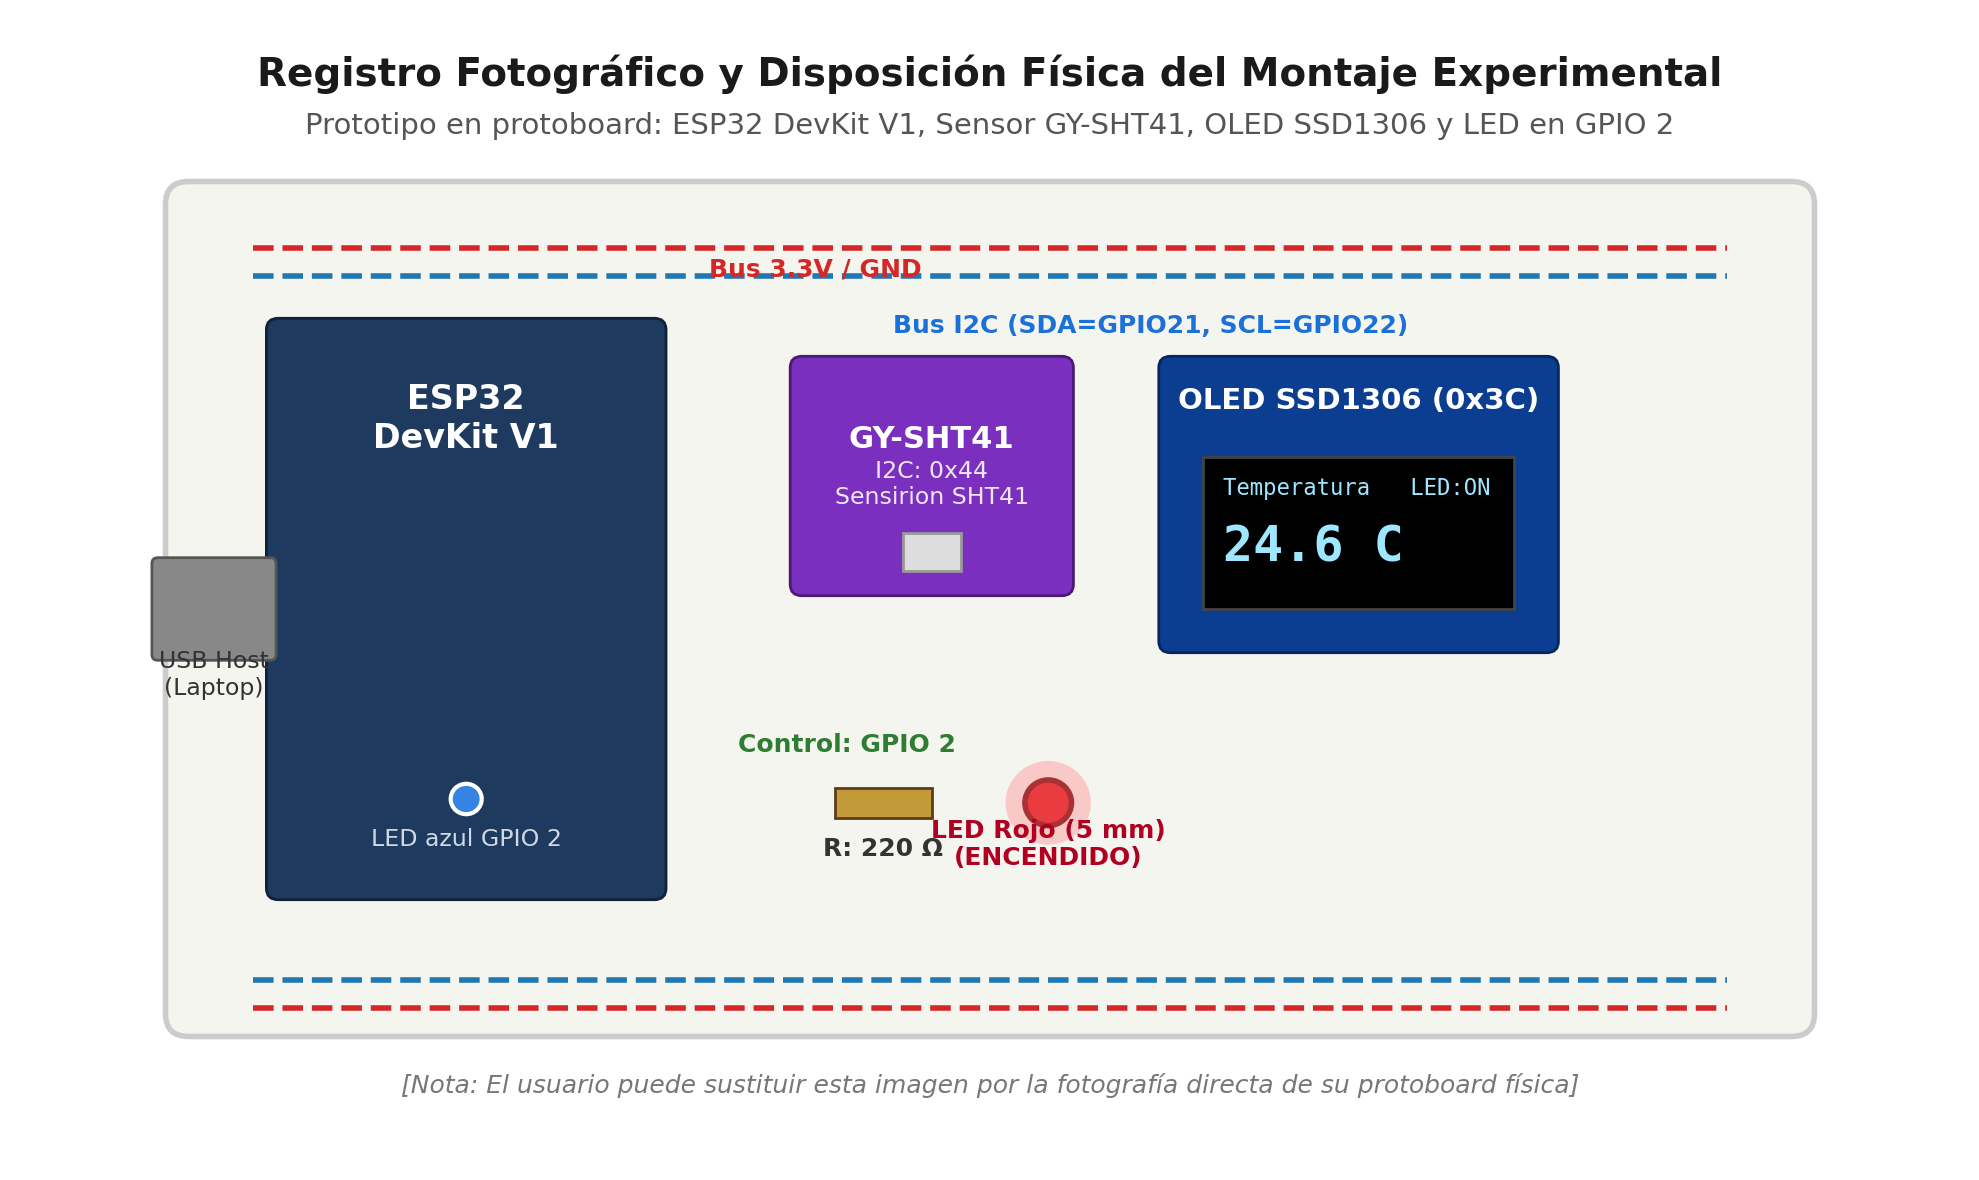
\includegraphics[width=\textwidth]{imagenes/evidencia_montaje_protoboard.png}
        \caption{Montaje experimental en protoboard.}
        \label{fig:sub_montaje}
    \end{subfigure}
    \hfill
    \begin{subfigure}[b]{0.48\textwidth}
        \centering
        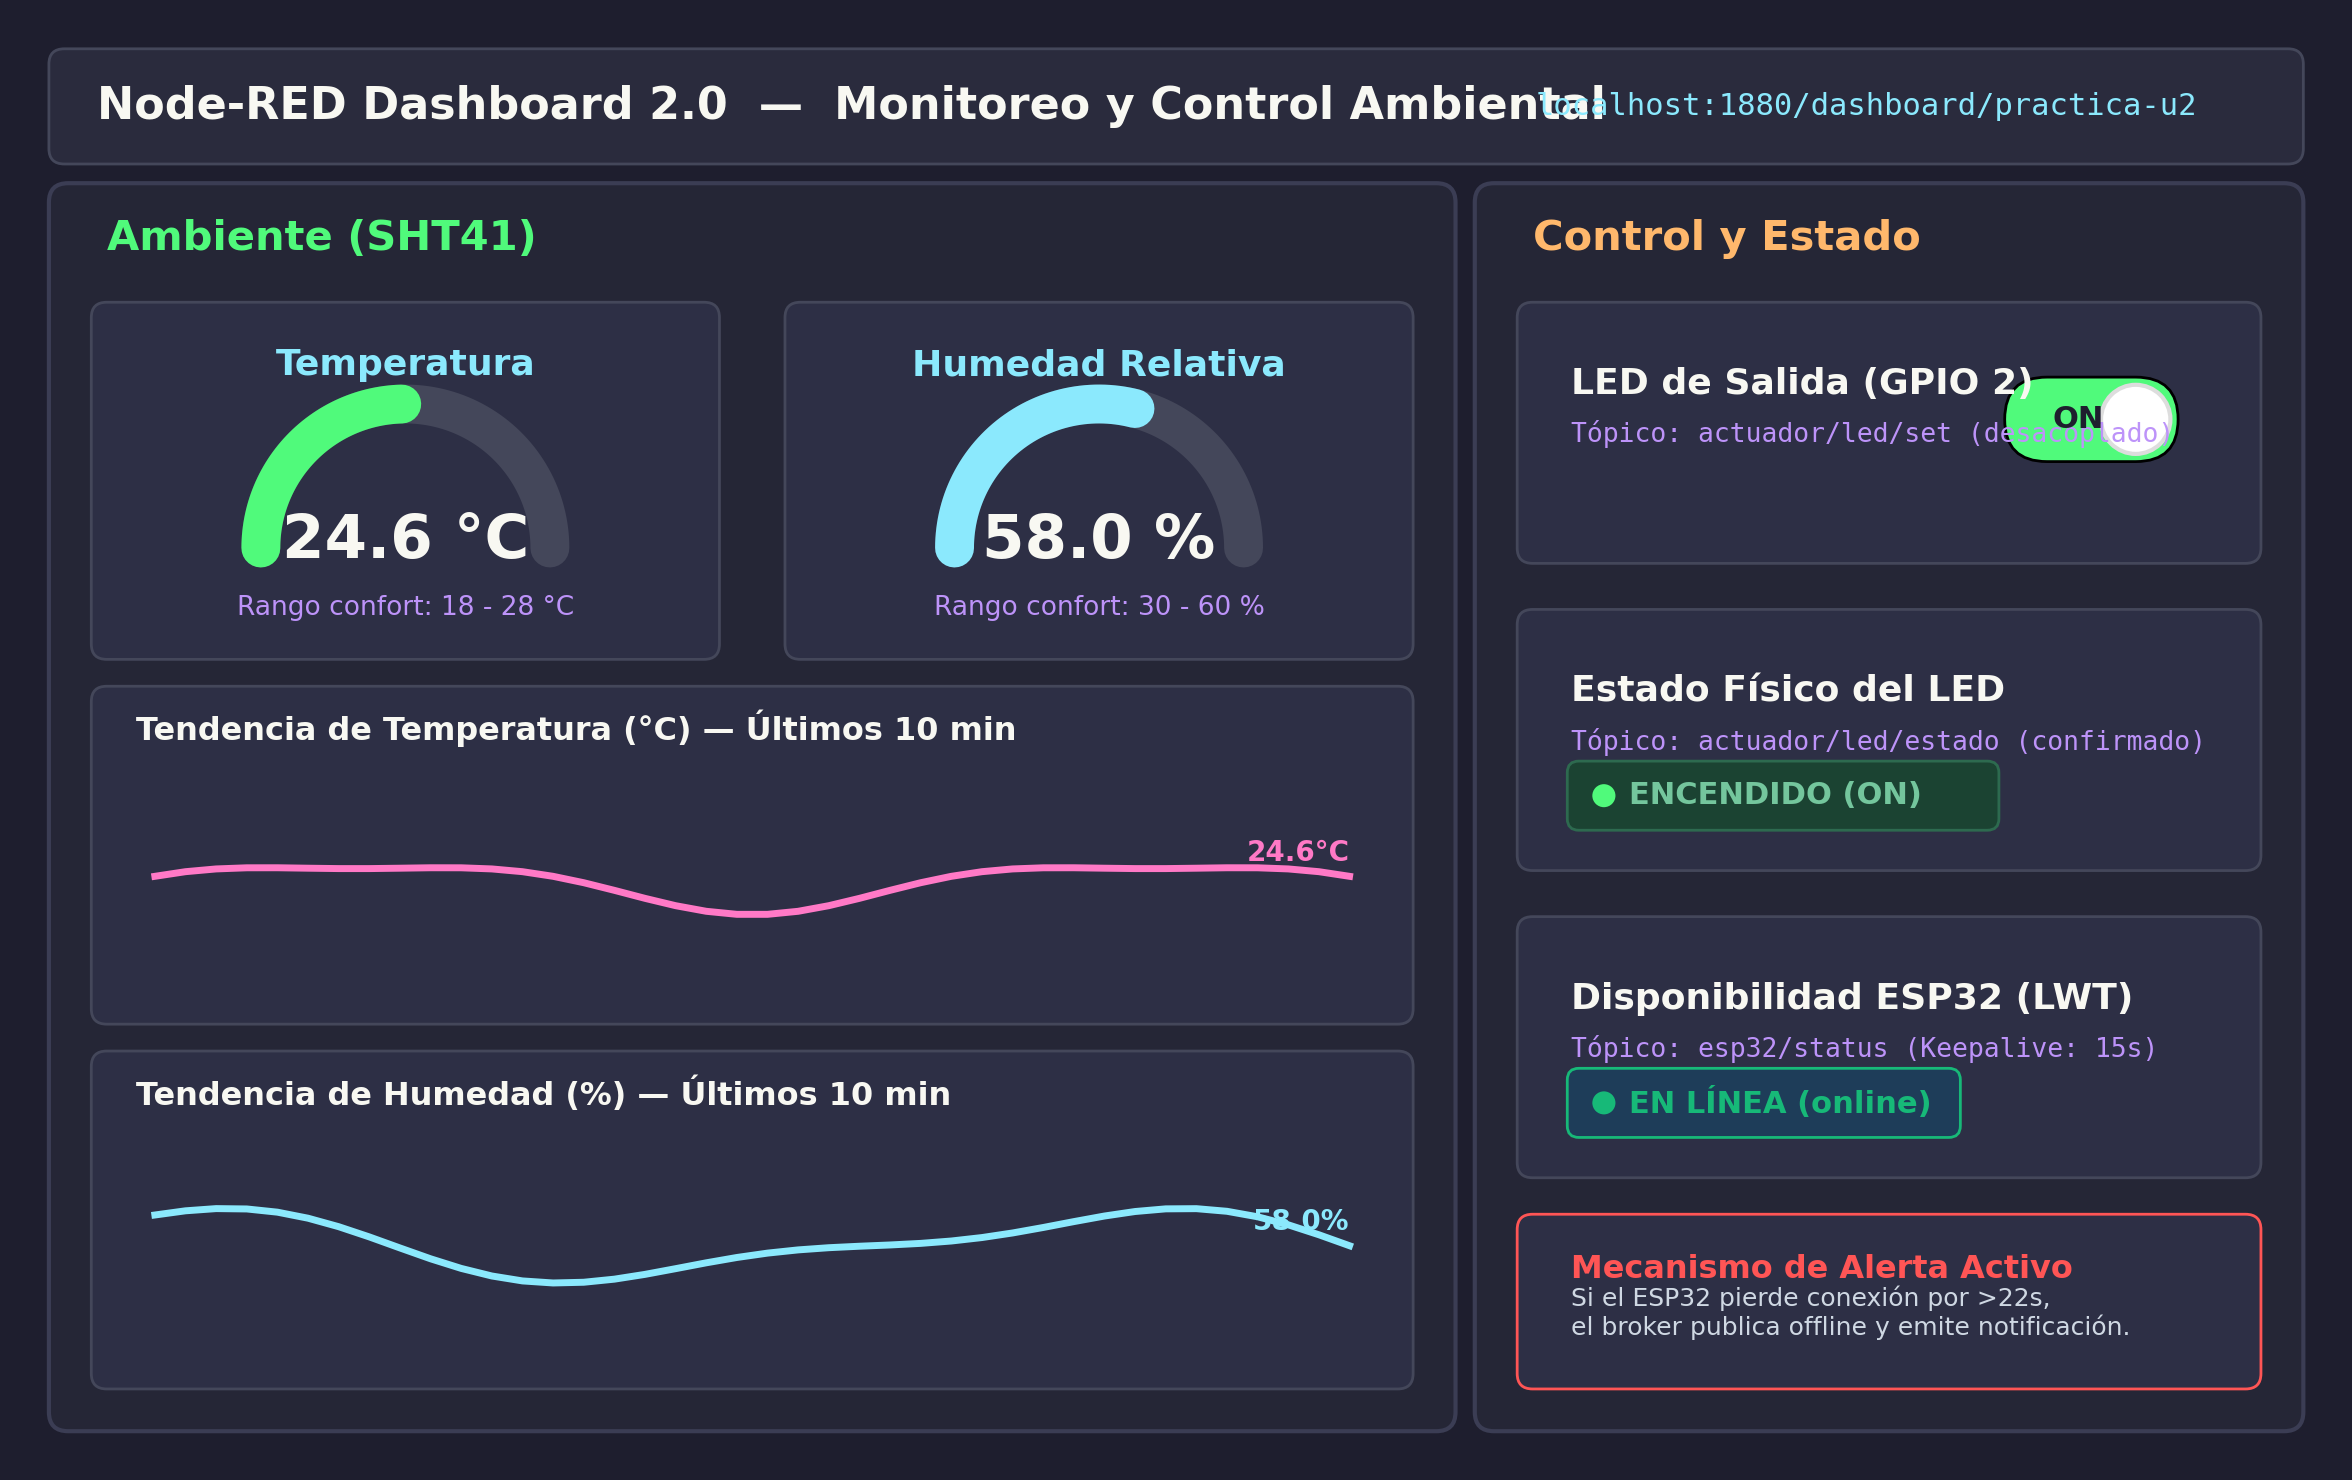
\includegraphics[width=\textwidth]{imagenes/dashboard_nodered.png}
        \caption{Dashboard 2.0 de Node-RED.}
        \label{fig:sub_dashboard}
    \end{subfigure}
    \caption{Evidencias de montaje físico y panel de supervisión web.}
    \label{fig:evidencias_visuales}
\end{figure}

\subsection{Demostración en Video}
\begin{infobox}[Video Demostrativo de Comunicación Bidireccional]
    \centering
    \textbf{Acceso al video demostrativo de pruebas experimentales:}\\
    \vspace{0.15cm}
    \url{https://drive.google.com/drive/folders/ejemplo-enlace-video-practica-u2}\\
    \vspace{0.15cm}
    \textit{\small(Demuestra la conmutación remota del LED, la actualización de la OLED y el reporte de LWT ante desconexiones).}
\end{infobox}

\subsection{Pruebas de Validación Experimental}
\begin{enumerate}
    \item \textbf{Secuencia de arranque en monitor serie (115200 bps):}
\begin{lstlisting}[style=custombash]
Conectando a WiFi: ESP32-Proyecto
WiFi conectado. IP del ESP32: 10.42.0.84
Conectando a broker MQTT... conectado.
Publicado en MQTT: {"temp":24.6,"hum":58.0}
Mensaje recibido [actuador/led/set]: ON
LED -> ON
\end{lstlisting}
    \item \textbf{Suscripción a telemetría desde terminal (CLI):}
\begin{lstlisting}[style=custombash]
$ mosquitto_sub -h 10.42.0.1 -u dashboard -P '<pass>' -v -t 'sensor/sht41/#' -t 'actuador/led/estado'
esp32/status online
actuador/led/estado OFF
sensor/sht41/temperatura 24.6
sensor/sht41/humedad 58.0
\end{lstlisting}
    \item \textbf{Control de actuador y confirmación de estado:} Al publicar \texttt{mosquitto\_pub -t actuador/led/set -m ON -q 1 -r}, el LED físico se enciende, la pantalla OLED muestra \texttt{LED:ON} y el ESP32 publica \texttt{actuador/led/estado ON}.
    \item \textbf{Verificación de LWT:} Al retirar la alimentación del ESP32, transcurridos 22 segundos el broker emite automáticamente \texttt{esp32/status offline}, actualizando el dashboard a \textbf{🔴 Desconectado}.
\end{enumerate}


% 11. PROBLEMAS ENCONTRADOS Y SOLUCIÓN
\section{Problemas Encontrados y Soluciones}

Durante el desarrollo del sistema se superaron diversos desafíos técnicos que se resumen en la Tabla~\ref{tab:problemas_solucion}.

\begin{table}[H]
\centering
\small
\begin{tabularx}{\textwidth}{p{3.8cm} p{5.2cm} X}
\toprule
\textbf{Problema Observado} & \textbf{Causa Raíz} & \textbf{Solución Implementada} \\
\midrule
Lecturas erróneas ($0^\circ\text{C}$) en sensor BME680 inicial & Falla interna en silicio: registro \texttt{adc\_T} en cero permanente & Sustitución por sensor industrial Sensirion GY-SHT41 (I²C). \\
\addlinespace
ESP32 retenido en reset al abrir monitor serie & Líneas DTR/RTS del convertidor USB (CH9102/CH343) forzaban pin EN & Configuración de \texttt{monitor\_rts = 0} y \texttt{monitor\_dtr = 0} en \texttt{platformio.ini}. \\
\addlinespace
ESP32 publica en MQTT pero Node-RED no recibe nada & Mosquitto descartaba tópicos en silencio por reglas ACL no actualizadas & Definición de reglas ACL por rol para \texttt{esp32\_user} y \texttt{dashboard} en \texttt{/etc/mosquitto/acl}. \\
\addlinespace
Nodos MQTT en Node-RED en \textit{"connecting"} tras importar & Flujo exportado omite credenciales por política de seguridad & Captura manual de usuario y contraseña en el nodo \texttt{Mosquitto local}. \\
\addlinespace
Colisión de URL en Dashboard 2.0 & Ruta \texttt{/monitoreo} ya utilizada en otra página & Reasignación de ruta a \texttt{/dashboard/practica-u2}. \\
\addlinespace
Bloqueo de escáner I²C en terminal & Cable jumper flojo forzaba línea SDA/SCL a tierra & Reemplazo de cable y aislamiento módulo por módulo. \\
\addlinespace
Desconexión de ESP32 al cambiar de red en laptop & La laptop apagaba el hotspot al asociarse a otra Wi-Fi & Asignación de IP fija \texttt{10.42.0.1/24} y reactivación unívoca con \texttt{nmcli}. \\
\bottomrule
\end{tabularx}
\caption{Problemas encontrados, causas y soluciones de ingeniería.}
\label{tab:problemas_solucion}
\end{table}


% 12. CONCLUSIONES
\section{Conclusiones}

\subsection{Conclusiones de la Práctica}
\begin{enumerate}[noitemsep]
    \item \textbf{Cumplimiento de la Comunicación Bidireccional:} Se validó exitosamente el intercambio simultáneo de telemetría ascendente (temperatura y humedad cada 2 segundos) y comandos descendentes de control (encendido/apagado del LED en GPIO 2) mediante MQTT sobre broker Mosquitto.
    \item \textbf{Robustez del Desacoplamiento de Estado:} El control en lazo cerrado implementado en Node-RED demostró que condicionar la interfaz gráfica a la confirmación real física (\texttt{actuador/led/estado}) previene discrepancias de estado si el dispositivo se apaga o pierde conectividad.
    \item \textbf{Detección Eficiente de Fallas con LWT:} La función Last Will and Testament permitió que el broker reporte automáticamente la desconexión del ESP32 sin necesidad de sobrecargar la red con mecanismos de sondeo continuo (\textit{polling}).
    \item \textbf{Programación No Bloqueante:} El uso de temporizadores cooperativos con \texttt{millis()} garantizó que las tareas locales (lectura de sensor y pantalla OLED) continúen ejecutándose fluidamente aun durante cortes o reconexiones de red.
\end{enumerate}

\subsection{Trabajo Futuro y Escalabilidad}
\begin{itemize}[noitemsep]
    \item \textbf{Migración a Nodo Autónomo Dedicado:} Trasladar Mosquitto y Node-RED de la laptop a una placa de bajo consumo (ej. \textbf{Orange Pi Zero 3}) que funcione como Access Point permanente y salida Ethernet hacia la red local.
    \item \textbf{Control de Cargas de Potencia:} Sustituir el LED por módulos de relé electromecánicos para control de ventilación o climatización (HVAC) con lógica automatizada en Node-RED.
    \item \textbf{Acceso Remoto Seguro:} Configurar una red privada virtual moderna tipo malla (\textbf{Tailscale} o \textbf{WireGuard}) para supervisión fuera de la red local sin exponer puertos a Internet.
\end{itemize}


\end{document}
